The success of transfer learning suggests that exploiting the knowledge of the existing models properly can greatly help us to learn new categories. 
Transfer learning on image recognition is a very popular topic in recent years. It is important for a classifier to learn the new categories continuously. To adapt multiple categories, the classifier can adapt one category each time iteratively, i.e.  extending the source $N$-category classifier to a target $N+1$ one.
Previous approaches show that, to add the new category to the existing classifier, leveraging the knowledge from source data and models can help this learning procedure effectively \cite{tommasi2014learning} \cite{kuzborskij2013n}. 
However, in some cases, we can only obtain the source models and it is difficult to access their training data.   
For instance, it becomes a common practice to reuse a trained object recognition model on new tasks without accessing the large-scale source image dataset.
Recently, some works have been proposed within a framework called Hypothesis Transfer Learning (HTL) to handle this situation \cite{kuzborskij2013stability}. HTL assumes only source models (called the hypothesis) trained on source task can be utilized and there is no access to source data, nor any knowledge about the relatedness of the source and target distributions. 

In HTL, a number of works have been attempted with Least Square Support Vector Machine (LS-SVM) \cite{kuzborskij2013stability}. Previous approaches show that the hypotheses can be evaluated effectively with LS-SVM via Leave-One-Out cross-validation \cite{tommasi2014learning}. The framework of HTL with LS-SVM has two major phrases: (I) Building binary One-Versus-All SVMs with transfer parameters. (II) Estimating the transfer parameters.
Previous methods of HTL assume that the hypotheses of the $N$ categories are correct for the corresponding categories in the target task, e.g. the source hypothesis to distinguish the orange and apple also works for the orange and apple in target task\cite{kuzborskij2013n}. However, the source hypothesis may fail in target task. For example, a source hypothesis is trained from to distinguish apple and orange using the images that are bright and have high contrast level, but the images of orange and apple collected by us could be low contrast and taken in a dark environment. Therefore, it is trivial to assume that the prior hypotheses are also correct for the data in the target task. 

In this paper, we extend previous methods by relaxing the assumption that the hypotheses from source task are correct the same category. 
When the source hypotheses fail, transferring from them could lead to negative transfer. 
In transfer learning, when the data distribution of the source and target task are similar, transferring the knowledge between them can improve the performance of the classifier for the target one, which is called positive transfer. On the other hand, when the data distribution is different, leveraging the knowledge could even degrade the performance of the classifier on target task, which is referred to as negative transfer \cite{pan2010survey}. 
In the worst case of HTL, where all hypotheses fail, transfer learning algorithms may suffer from negative transfer due to the mismatched data distribution. In our case, this mismatched distribution can result from both the $N$ original categories and the newly added category (see Figure \ref{fig:distribution}). 

%Previous works \cite{tommasi2014learning}, \cite{kuzborskij2013n} suggest that to better utilizing the hypotheses and reduce negative transfer, the decision of the algorithm should be made by combining the prior hypotheses and empirical knowledge (from the specific target task).

%\begin{figure}
%\centering
%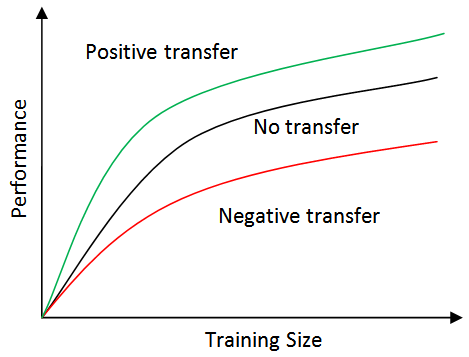
\includegraphics[scale=.5]{fig/negative.png}
%\caption{Positive transfer VS Negative transfer. %Relying on unrelated prior knowledge too much could %lead to negative transfer.}\label{fig:neg}
%\end{figure}
\begin{figure}
\centering
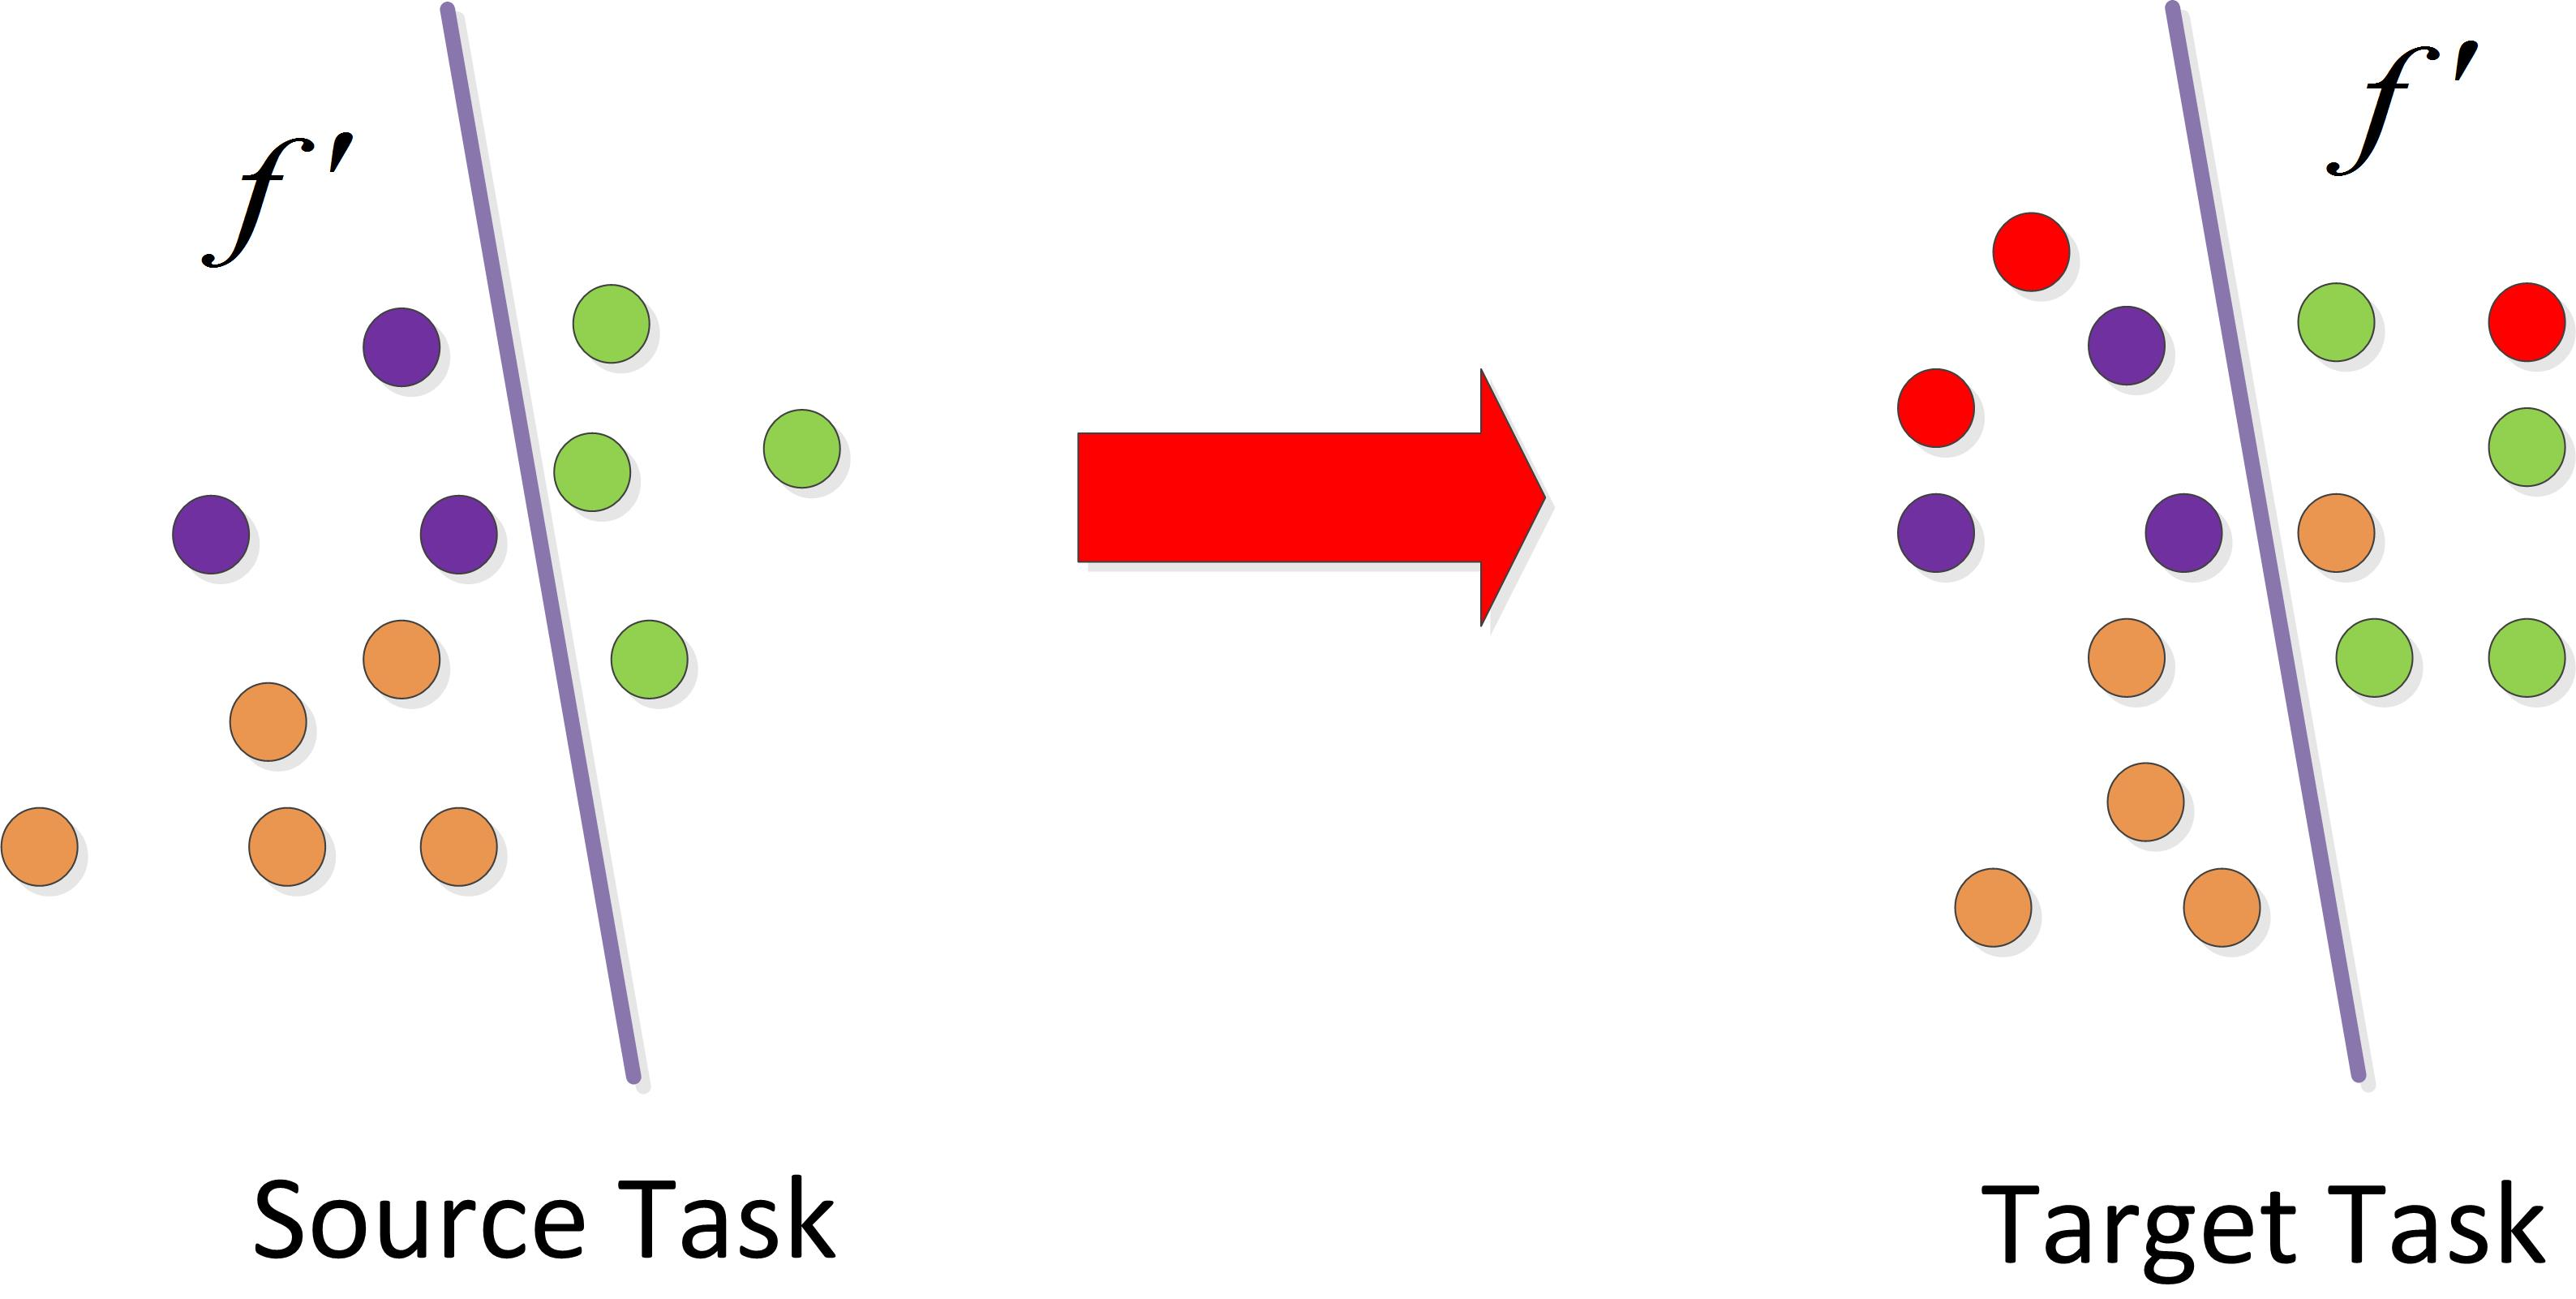
\includegraphics[scale=.4]{fig/domain.jpg}
\caption{Negative transfer happens when we transfer prior hypothesis $f'$ to target one. Points with different color represent different categories. The data distribution would change even for identical categories in different task. The new added category (red points) can also greatly affect the data distribution in target task. }\label{fig:distribution}
\end{figure}

%How to safely utilize the hypotheses to avoid negative transfer is still an open question in transfer learning \cite{Lu201514}. Previous works of HTL use Leave-One-Out error to avoid negative transfer \cite{tommasi2014learning}\cite{kuzborskij2013n}.
Previous methods of HTL focus on how to leverage the knowledge for the new category and are not able to avoid negative transfer, especially when all the hypotheses fails (see experiments in Section \ref{sec:exp}).
In this paper, we propose our method, called Safety Multiclass Incremental Transfer Learning (SMITLe), that can both avoid negative transfer and leverage correct hypotheses. 
The main contributions of this paper include: (1) We propose a novel algorithm SMITLe within the HTL framework that can safely utilize the prior hypotheses to prevent negative transfer. (2) We also show that SMITLe can obtain the optimal solution at the rate of $O(\frac{\log(t)}{t})$ where $t$ is training iteration. 
Following the two phrases of HTL, in Phrase I, to train the binary models for the target task, we propose an objective function with transfer parameters that can control the amount of knowledge from the hypotheses. 
%a regularization term adopted from Multi-KT \cite{tommasi2014learning} is used to adapt the $N$ original categories and the new category. As a result, the decision of each binary LS-SVM is the linear combination of the prior hypotheses and empirical knowledge (from target data) controlled by some transfer parameters. 
In Phrase II, to measure the transferability of each prior hypothesis, we estimate our transfer parameters using multi-class prediction error based on closed-form leave-one-out (LOO) error for model evaluation.
Moreover, we propose our novel objective function that can balance the weight between the prior hypotheses and empirical knowledge from target task. We prove that transfer parameters learned from our novel objection function can avoid negative transfer. Experimental results show that SMITLe can achieve better accuracy than other existing baselines.

The rest of this paper is organized as follow.
In Section \ref{sec:prob}, we introduce the biased regularization terms of our problem for phrase 1 of HTL. Then, we propose a novel objective function for transfer parameter estimation, called SMITLe in Section \ref{sec:smitle}. We show that the estimated transfer parameter can distinguish the utility of the prior hypothesis and avoid negative transfer autonomously. In Section \ref{sec:exp}, we show the performance comparison between SMITLe and other baselines on a variety of experiments on AwA and Caltech datasets in three different scenarios.
